\documentclass[11pt,a4paper]{article}

\usepackage[margin=2.3cm]{geometry}
\usepackage[T1]{fontenc}
\usepackage{lmodern}
\usepackage{graphicx}
\usepackage{booktabs}
\usepackage{tabularx}
\usepackage{array}
\usepackage{float}
\usepackage{caption}
\usepackage{xcolor}
\usepackage{enumitem}
\usepackage{amsmath}
\usepackage{tikz}
\usetikzlibrary{positioning,arrows.meta}
\usepackage[hidelinks]{hyperref}

\graphicspath{{figures/}}
\setlist{nosep}
\setlength{\parskip}{0.5em}
\setlength{\parindent}{0pt}
\captionsetup{font=small,labelfont=bf}

\newcommand{\ugm}{\,$\mu$g/m$^{3}$}
\newcommand{\tofill}[1]{\textcolor{red}{\textbf{[FILL IN FROM KAGGLE RUN LOG: #1]}}}
\newcolumntype{L}{>{\raggedright\arraybackslash}X}

\begin{document}

%-------------------------------------------------------------------- Title
\begin{titlepage}
\centering
{\large Uganda Christian University\par}
{\large Faculty of Engineering, Design and Technology\par}
{\large Department of Computing and Technology\par}
\vspace{1.5cm}
{\large CSC3119: AI Model Deployment and Scalability\par}
{\large Track: Artificial Intelligence and Robotics\par}
\vspace{1.5cm}
{\Huge\bfseries Predicting PM2.5 Air Quality Concentrations from AirQo Sensor Data\par}
\vspace{0.8cm}
{\Large Assignment 4: Final Report\par}
\vspace{1.5cm}
\begin{tabular}{rll}
\toprule
No. & Name & Registration No. \\
\midrule
1 & Charis Opol & S24B23/003 \\
2 & Kirabo Esther Kebirungi & S24B23/045 \\
3 & Ansasiire Nehum Naamaye & S24B23/018 \\
4 & Norah-Angel Nakaye & M24B23/008 \\
5 & Mwonge Andrea & S24B23/070 \\
6 & Cole Rodney Migisha & S24B23/006 \\
7 & Ssendagire Abubaker & S24B23/012 \\
8 & Shane Munanura & M24B23/031 \\
9 & Mirembe Peace Mercy & M24B23/005 \\
10 & Tony Blair & S24B23/024 \\
11 & Musoke Nestroy & S24B23/069 \\
\bottomrule
\end{tabular}
\vfill
{\large October 2026\par}
\end{titlepage}

%-------------------------------------------------------------------- Abstract
\begin{abstract}
We built a complete pipeline that predicts hourly PM2.5 concentration from AirQo low-cost sensor data: data preparation, exploratory analysis, model training and tuning, August 2026 forecasts, monitoring with Evidently AI, and deployment. The supplied data contains 14{,}600 hourly records from 149 sensors, but genuine readings exist on only eight days (1--3 January, 1--2 April and 1--3 June 2026), and about 28\% of AirQo records report physically impossible zero temperature and humidity. Zeros were treated as missing, each sensor was resampled to a complete hourly grid, and PM2.5 targets were never imputed. Six regression models were tuned with time-ordered cross-validation on a Z-score target. A tuned Random Forest performed best on the held-out June period (MAE 3.10\ugm, RMSE 7.00\ugm, $R^2$ 0.898) and assigns the correct AQI category to 86.2\% of test hours. Most of this skill comes from PM10 measured at the same hour, which is not known in advance, so the August forecasts represent each sensor's typical daily pattern rather than reacting to future conditions. The pipeline was verified locally, then deployed and run end to end in the cloud on Kaggle, and the model and an interactive forecast demo were published on Hugging Face.
\end{abstract}

\tableofcontents
\newpage

%==================================================================== 1
\section{Introduction}

AirQo, based at Makerere University, operates a network of locally manufactured low-cost air-quality monitors across African cities. Fine particulate matter (PM2.5) is the pollutant of greatest health concern: the particles penetrate deep into the lungs and bloodstream, and a four-year reference-grade study cited in the assignment brief found Kampala's annual average to be about 39\ugm{}, roughly eight times the WHO annual guideline of 5\ugm{}~\cite{who2021}. Forecasting PM2.5 supports early warnings for the public and health services, and planning by NEMA and the ministries responsible for energy and transport.

The assignment asks for a deployable pipeline that goes from raw sensor data to a trained, evaluated, monitored and cloud-deployed model. This report documents each stage, the decisions taken and the evidence behind them. The AQI categories used throughout are those of Section~4 of the brief (Table~\ref{tab:aqi}).

\begin{table}[H]
\centering
\caption{PM2.5 AQI categories used throughout the project.}
\label{tab:aqi}
\begin{tabular}{ll}
\toprule
PM2.5 (\ugm) & Category \\
\midrule
0 -- 9 & Good \\
9.101 -- 35.49 & Moderate \\
35.491 -- 55.49 & Unhealthy for Sensitive Groups (USG) \\
55.491 -- 125.49 & Unhealthy \\
125.491 -- 225.49 & Very Unhealthy \\
above 225.49 & Hazardous \\
\bottomrule
\end{tabular}
\end{table}

%==================================================================== 2
\section{Methodology overview}

Figure~\ref{fig:pipeline} shows the pipeline. All stages are implemented in a single notebook, \texttt{train.ipynb}, which runs unattended from start to finish so that exactly the same code runs locally and on the cloud.

\begin{figure}[H]
\centering
\begin{tikzpicture}[
  node distance=0.45cm and 0.9cm,
  box/.style={draw, rounded corners, fill=blue!6, align=center, text width=4.6cm, minimum height=0.9cm, font=\small},
  out/.style={draw, rounded corners, fill=green!8, align=center, text width=4.6cm, minimum height=0.9cm, font=\small},
  arr/.style={-{Stealth[length=2.2mm]}, thick}
]
\node[box] (raw) {\textbf{Raw data}\\14{,}600 hourly records, 149 sensors};
\node[box, below=of raw] (clean) {\textbf{Cleaning}\\zeros $\rightarrow$ missing, types, coordinates};
\node[box, below=of clean] (resample) {\textbf{Hourly resampling}\\complete Jan--Jul grid per sensor};
\node[box, below=of resample] (interp) {\textbf{Short-gap interpolation}\\predictors only, gaps $\le$ 3 h};
\node[box, below=of interp] (eda) {\textbf{EDA}\\5 Kampala sensors, AQI bands, Z-score};
\node[box, below=of eda] (feat) {\textbf{Features and split}\\cyclical time, chronological split};

\node[box, right=of raw] (train) {\textbf{Train and tune}\\6 models, TimeSeriesSplit CV};
\node[box, below=of train] (select) {\textbf{Evaluate and select}\\MAE, RMSE, $R^2$, AQI accuracy};
\node[box, below=of select] (save) {\textbf{Serialise}\\\texttt{best\_pm25\_model.joblib}};
\node[box, below=of save] (fc) {\textbf{Forecast}\\1--14 Aug daily, 1 Aug hourly};
\node[box, below=of fc] (mon) {\textbf{Monitor}\\Evidently data and model drift};
\node[out, below=of mon] (dep) {\textbf{Deploy}\\Kaggle cloud run; Hugging Face demo};

\foreach \a/\b in {raw/clean, clean/resample, resample/interp, interp/eda, eda/feat, train/select, select/save, save/fc, fc/mon, mon/dep}
  \draw[arr] (\a) -- (\b);
\draw[arr] (feat.east) -- ++(0.45,0) |- (train.west);
\end{tikzpicture}
\caption{Methodology pipeline, from raw sensor data to deployment.}
\label{fig:pipeline}
\end{figure}

%==================================================================== 3
\section{Data}

The dataset (\texttt{Sensor Data Jan - July 2026.csv}) contains 14{,}600 hourly records with 12 fields: site name, timestamp, sample frequency, network (AirQo or AirGradient), latitude, longitude, temperature, humidity, calibrated PM2.5 and PM10, site ID and device name. It covers 149 devices at 145 named sites. There are no duplicate rows and no duplicate device-hour pairs, so \texttt{device\_name} together with the timestamp uniquely identifies an observation.

Three properties of the data shaped every later decision:

\begin{enumerate}
\item \textbf{Very sparse coverage in time.} Although the file is named January--July, genuine readings exist on only eight days, in three short windows: 1--3 January, 1--2 April and 1--3 June 2026. The last reading is at 03:00 UTC on 3 June. Between windows, sensors are offline for up to 150 days.
\item \textbf{Zero values that are not real readings.} The brief defines 0 or empty as missing for temperature, humidity, PM2.5, PM10, latitude and longitude. Table~\ref{tab:missing} shows how common these are.
\item \textbf{Uneven sensors.} Devices contribute between 20 and 147 records (median 105). Three sites host more than one device.
\end{enumerate}

\begin{table}[H]
\centering
\caption{Null and zero values in the raw data. Zeros are treated as missing, as the brief requires.}
\label{tab:missing}
\begin{tabular}{lrrr}
\toprule
Field & Empty & Zero & Total missing \\
\midrule
Latitude & 1 & 3{,}085 & 3{,}086 \\
Longitude & 0 & 3{,}067 & 3{,}067 \\
Temperature & 54 & 4{,}066 & 4{,}120 \\
Humidity & 206 & 4{,}159 & 4{,}365 \\
PM2.5 (target) & 325 & 0 & 325 \\
PM10 & 427 & 3 & 430 \\
\bottomrule
\end{tabular}
\end{table}

%==================================================================== 4
\section{Data preparation}

\subsection{Approach and supporting literature}

The preparation follows the general workflow of Febrian and Permai~\cite{febrian2025}: standardise null values, quantify missingness, explore distributions and outliers, analyse correlations, impute where justified, normalise, and split chronologically for forecasting. AirQo's own studies describe the same characteristics we found in this data: intermittent device availability, varying data completeness, and calibrated PM values from low-cost sensors~\cite{okure2022,sserunjogi2022}. Because of that, we did not copy imputation choices mechanically from other datasets. In particular, the Jakarta study imputes with interpolation and KNN, but filling missing PM2.5 \emph{targets} here would create artificial labels and bias the models, so targets are never imputed.

\subsection{Null standardisation and data types}

All zeros in the six fields of Table~\ref{tab:missing} were converted to missing values. Timestamps were parsed as UTC datetimes, measurement fields as nullable floats, and identifiers (\texttt{site\_id}, \texttt{site\_name}, \texttt{device\_name}) as strings. \texttt{site\_id} is missing in about half the rows, so \texttt{device\_name}, which is always present and unique per sensor, is used as the sensor identifier.

\subsection{The zero temperature and humidity readings}

About 4{,}100 rows report 0\,\textdegree C and 0\% humidity, values that are physically impossible in Uganda. The pattern shows a weather-sensor dropout rather than real readings:
\begin{itemize}
\item every zero temperature coincides with a zero humidity;
\item within a sensor the zeros come in long, unbroken blocks;
\item they occur only on AirQo devices (28.8\% of their rows), never on AirGradient devices.
\end{itemize}

For cleaning and EDA these values are missing, so they never enter statistics, plots or the Z-score. For the model inputs we tested several treatments (Table~\ref{tab:zeros}) and found the choice makes almost no difference: PM10 dominates the model (Section~\ref{sec:importance}), and temperature and humidity carry about 1\% of the importance each. The final pipeline encodes a missing weather value as 0, a constant ``sensor dropout'' marker that a tree model can recognise. We also tested filling dropouts from neighbouring sensors within 10\,km at the same hour; it reproduced real readings to within 1.0\,\textdegree C and 4.5\% humidity, but did not improve accuracy.

\begin{table}[H]
\centering
\caption{Effect of the zero-value treatment on test MAE (Random Forest baseline, 200 trees, same chronological split).}
\label{tab:zeros}
\begin{tabular}{lr}
\toprule
Treatment of missing temperature, humidity and PM10 & Test MAE (\ugm) \\
\midrule
Missing, median-imputed (with latitude/longitude as features) & 3.24 \\
Missing, median-imputed (no coordinates) & 3.30 \\
Kept as 0 & 3.24 \\
Median-imputed plus a ``dropout'' flag & 3.29 \\
Temperature and humidity removed entirely & 3.54 \\
\midrule
Ridge regression: median-imputed vs.\ kept as 0 & 5.35 vs.\ 5.33 \\
\bottomrule
\end{tabular}
\end{table}

\subsection{Coordinates}

Coordinates are a fixed property of a site, so missing values were filled with the median of the site's own valid coordinates, which is robust to the occasional bad GPS fix. Six sites never recorded a valid coordinate. We deliberately left these missing rather than inventing positions, because sensors with similar pollution profiles are not necessarily close together.

\subsection{Hourly resampling}

Each sensor was reindexed to a complete hourly grid from 1 January 00:00 to 31 July 23:00 UTC (5{,}088 hours). The resulting table has 758{,}112 rows (149 sensors $\times$ 5{,}088 hours), of which 743{,}512 are offline hours that now appear explicitly as missing rather than being absent. Fixed sensor attributes (site, network, coordinates) are carried onto the new rows. An \texttt{is\_offline} flag records which rows were added.

\subsection{Interpolation}

Most gaps between consecutive readings are one hour (13{,}668 cases), but 783 are longer, up to 150 days. Only short \emph{interior} gaps of at most three hours were linearly interpolated, and only for the predictors (temperature, humidity, PM10). Longer gaps stay missing to represent genuine sensor downtime. PM2.5 was never interpolated.

\subsection{Feature selection}

\begin{itemize}
\item \textbf{Kept:} temperature and humidity (the brief notes they influence PM2.5 through boundary-layer height and particle growth), PM10, and the device identifier.
\item \textbf{Time features:} hour of day, day of week and month, each encoded as a sine/cosine pair so that, for example, 23:00 and 00:00 are close.
\item \textbf{Dropped:} latitude and longitude, because \texttt{device\_name} already identifies each location; and administrative fields (frequency, network, site ID), which carry no predictive information.
\end{itemize}

%==================================================================== 5
\section{Exploratory data analysis}

\subsection{Sensor selection}

EDA focuses on five sensors inside Kampala District, as the brief requires. Instead of choosing sites by hand, we ranked single-device Kampala sites by the number of hours with all four measurements present and took the top five (Table~\ref{tab:sites}). Sites with several co-located devices were excluded so that each site is one clean time series. Nsasa (Kira Municipality) had more data than Kabusu but lies in Wakiso, outside Kampala, so it was excluded.

\begin{table}[H]
\centering
\caption{The five Kampala sensors used for EDA.}
\label{tab:sites}
\begin{tabular}{llrr}
\toprule
Site & Device & PM2.5 records & Complete records \\
\midrule
Nakasero II, Kampala & \texttt{aq\_66} & 147 & 147 \\
Lower Nsooba, Kawempe & \texttt{aq\_g507} & 144 & 144 \\
Salama Road & \texttt{ag\_588c81267534} & 142 & 142 \\
Namungona Primary School & \texttt{airqo\_g5365} & 135 & 135 \\
Kabusu, Natete Road & \texttt{aq\_g5\_100} & 134 & 134 \\
\bottomrule
\end{tabular}
\end{table}

\subsection{Distributions and outliers}

Across all 14{,}275 genuine PM2.5 readings, the mean is 32.7\ugm{} (standard deviation 30.4\ugm), ranging from 4.3 to 998.4\ugm. The distribution is strongly right-skewed (Figure~\ref{fig:dist}): most hours are Moderate, with a long tail of pollution episodes.

Outliers were flagged with sensor-specific IQR limits (values beyond $Q_1-1.5\,\mathrm{IQR}$ or $Q_3+1.5\,\mathrm{IQR}$ for that sensor), because sites have very different typical levels. This flagged 652 readings (4.6\%); Figure~\ref{fig:box} shows them per Kampala sensor. Thirteen readings exceed 200\ugm. Most are plausible episodes with PM10 rising alongside (for example 290\ugm{} at Salama Road on 1 January). The maximum, 998.4\ugm{} at Nansana with PM10 of only 70.8\ugm, is physically suspicious. Outliers were \textbf{flagged and retained}, because extreme values may be genuine pollution events and the brief asks for their treatment to be tracked rather than silently removed.

Two physical-consistency checks were also logged. PM2.5 exceeds PM10 in 22.4\% of comparable rows, which should not happen physically and points to calibration differences between the two channels. And 219 PM10 readings (1.5\%) are below 1\ugm. These rows are flagged, not removed.

\begin{figure}[H]
\centering
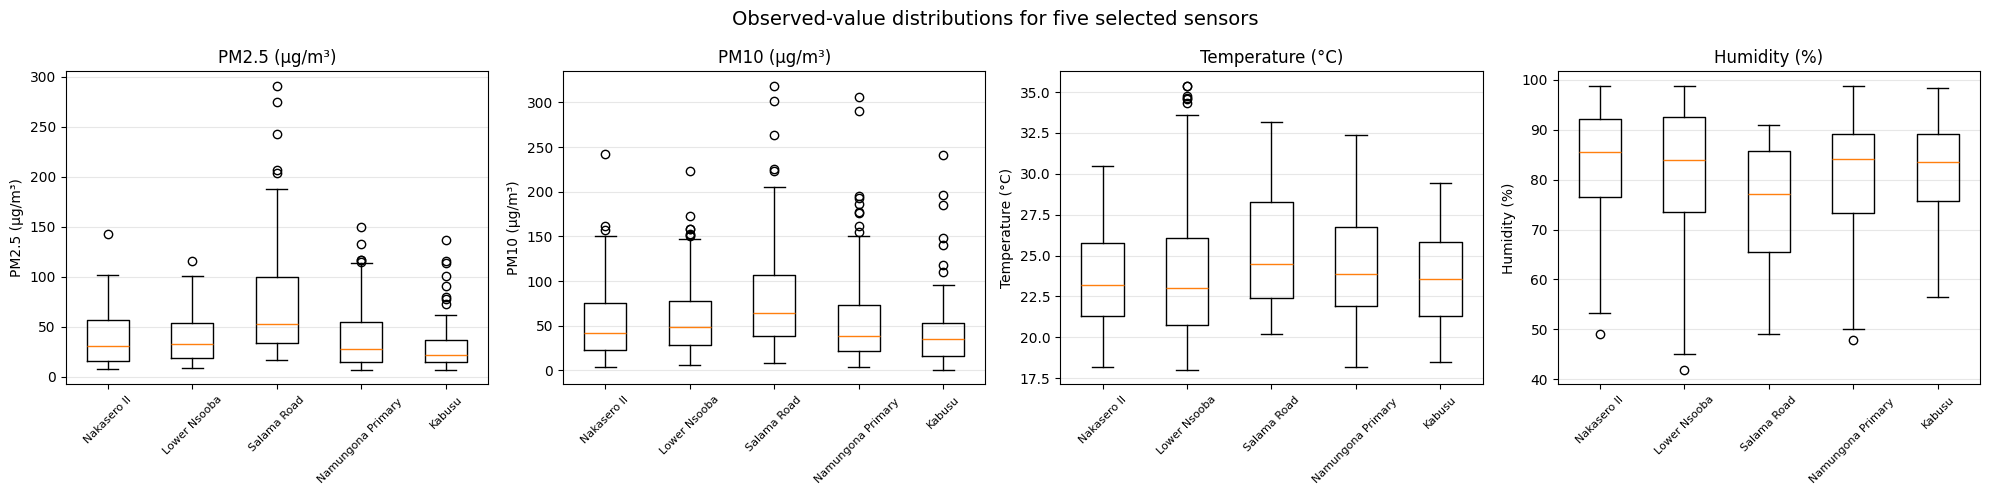
\includegraphics[width=\textwidth]{eda_boxplots.png}
\caption{Box plots of PM2.5, PM10, temperature and humidity for the five Kampala sensors. Salama Road has the highest and most variable PM2.5.}
\label{fig:box}
\end{figure}

\begin{figure}[H]
\centering
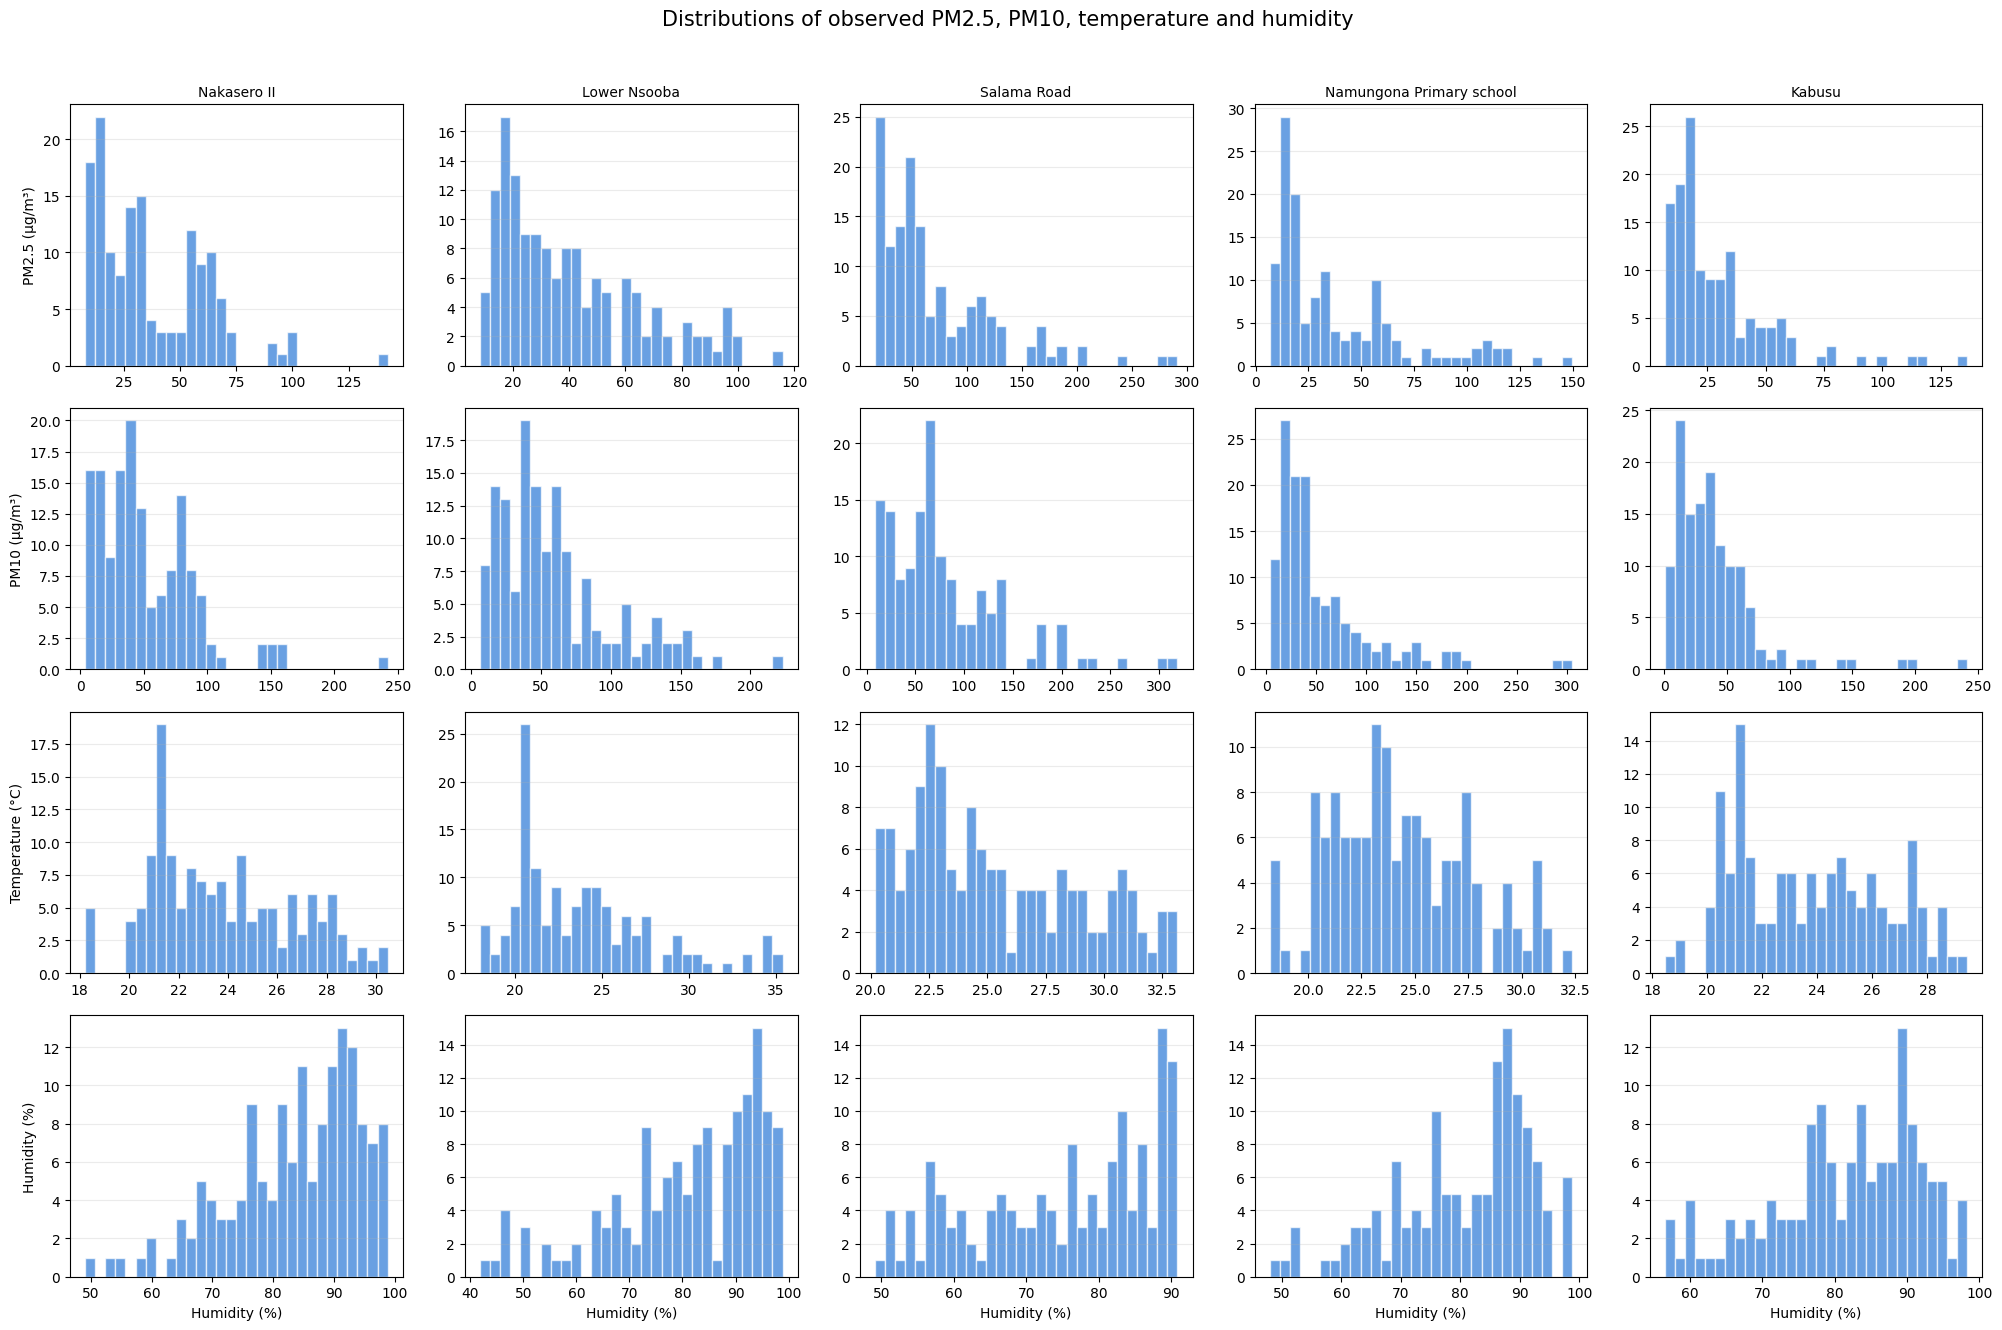
\includegraphics[width=\textwidth]{eda_distributions.png}
\caption{Distributions of the four measurements for each Kampala sensor (genuine readings only).}
\label{fig:dist}
\end{figure}

\subsection{AQI categories}

Of the 14{,}275 genuine readings, 1{,}249 are Good, 8{,}494 Moderate, 1{,}820 Unhealthy for Sensitive Groups, 2{,}565 Unhealthy, 137 Very Unhealthy and 10 Hazardous. Only 8.7\% of hours meet the ``Good'' threshold.

\subsection{Calendar and time-series plots}

Because readings exist on only eight days, a January-to-June calendar would be almost entirely blank. Both the calendar (Figure~\ref{fig:cal}) and the time series (Figure~\ref{fig:ts}) are therefore split into the three observation windows, each coloured by the AQI categories. Cells in the calendar show the daily mean and the number of hourly readings behind it, since days with few readings (3 January has one or two) are weaker estimates.

\begin{figure}[H]
\centering
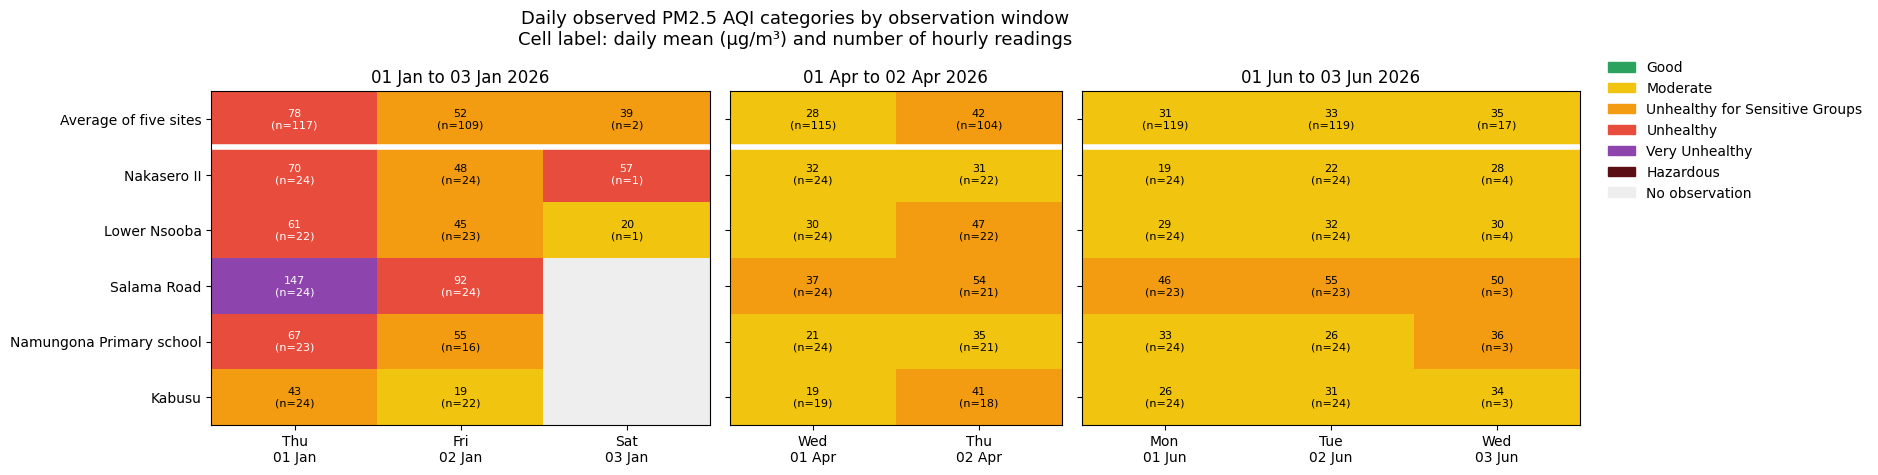
\includegraphics[width=\textwidth]{eda_calendar.png}
\caption{Calendar of daily mean PM2.5 (unscaled, cleaned) by observation window, coloured by AQI category. Early January was the most polluted window, with Salama Road reaching Very Unhealthy.}
\label{fig:cal}
\end{figure}

\begin{figure}[H]
\centering
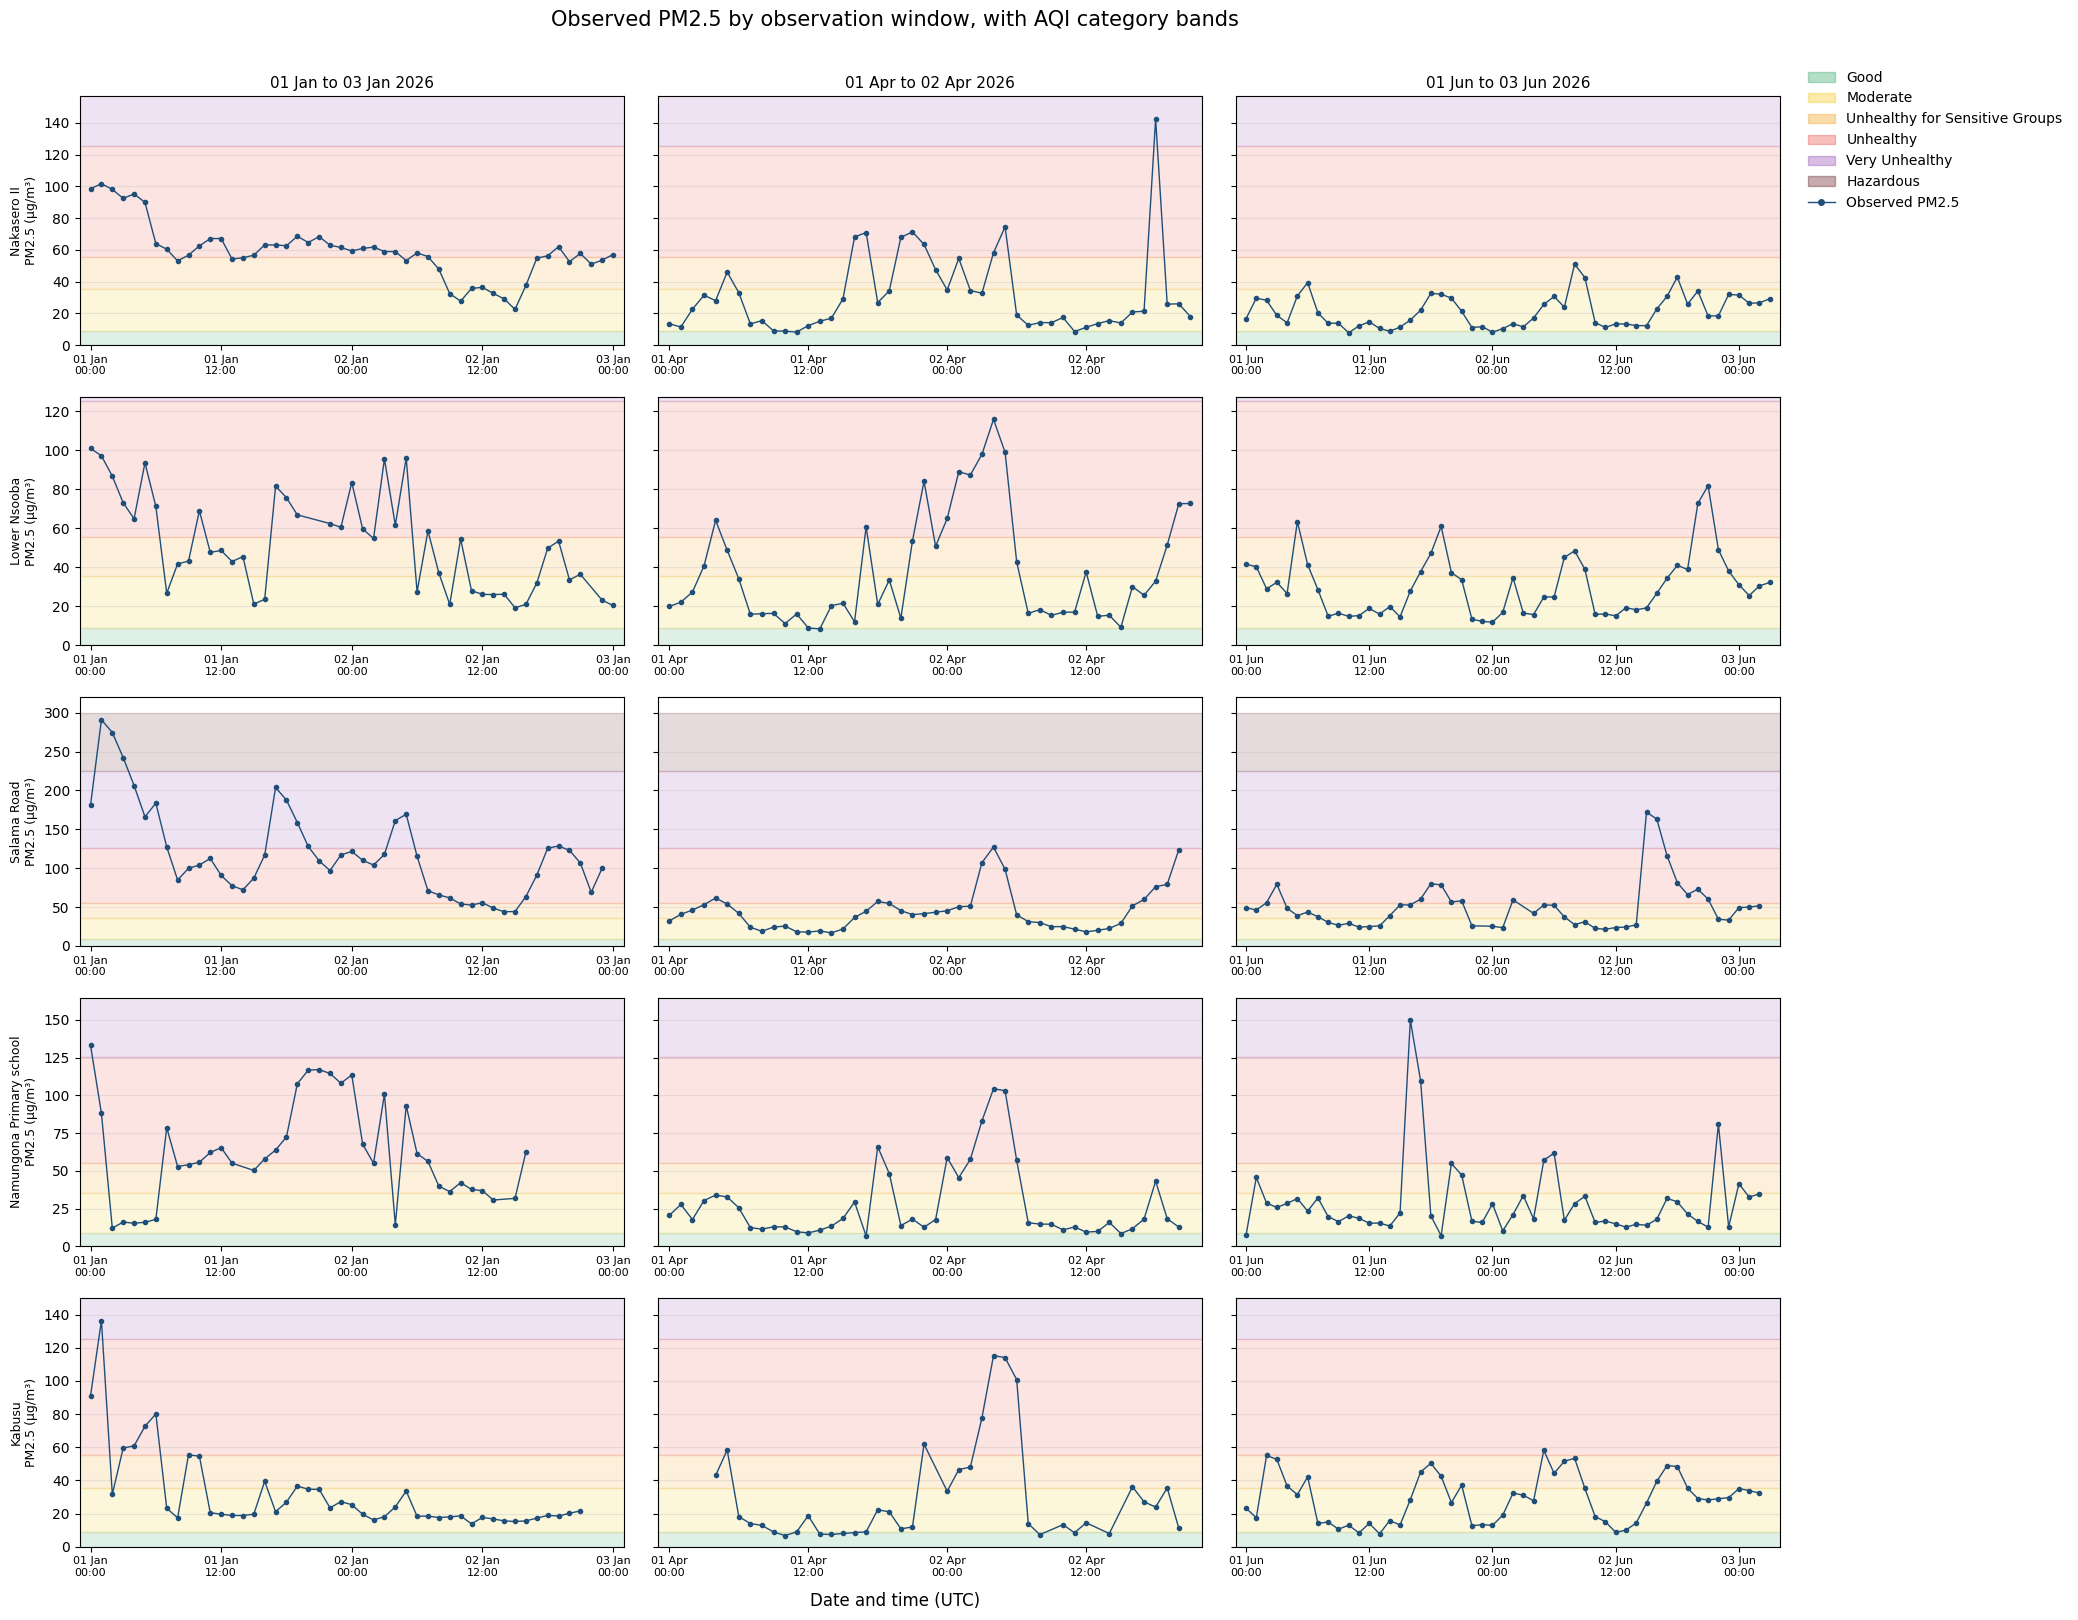
\includegraphics[width=\textwidth]{eda_timeseries.png}
\caption{Hourly PM2.5 for the five Kampala sensors in each observation window, with AQI categories as shaded background bands. Peaks recur in the early morning and evening, consistent with traffic and temperature inversions.}
\label{fig:ts}
\end{figure}

\subsection{Correlation with temperature and humidity}

Table~\ref{tab:corr} and Figures~\ref{fig:scatter}--\ref{fig:corrmat} show the relationship between PM2.5 and the weather variables. At every site, PM2.5 is negatively correlated with temperature ($r$ from $-0.13$ to $-0.51$) and positively with humidity ($r$ from $0.08$ to $0.43$). This agrees with the mechanism described in the brief: cool, humid hours (night and early morning) have a shallow boundary layer that traps pollutants, while warm afternoons mix them away. Temperature and humidity are themselves strongly anti-correlated ($r \approx -0.9$), so they carry largely the same information. PM2.5 and PM10 are almost perfectly correlated at every site ($r$ between 0.95 and 1.00), which foreshadows PM10's dominance in the models.

\begin{table}[H]
\centering
\caption{Pearson correlation of PM2.5 with temperature and humidity (genuine paired readings).}
\label{tab:corr}
\begin{tabular}{lrrr}
\toprule
Site & $r$ (temperature) & $r$ (humidity) & Pairs \\
\midrule
Nakasero II & $-0.133$ & $0.155$ & 147 \\
Lower Nsooba & $-0.321$ & $0.354$ & 144 \\
Salama Road & $-0.508$ & $0.411$ & 142 \\
Namungona Primary School & $-0.217$ & $0.079$ & 135 \\
Kabusu, Natete Road & $-0.469$ & $0.431$ & 134 \\
\bottomrule
\end{tabular}
\end{table}

\begin{figure}[H]
\centering
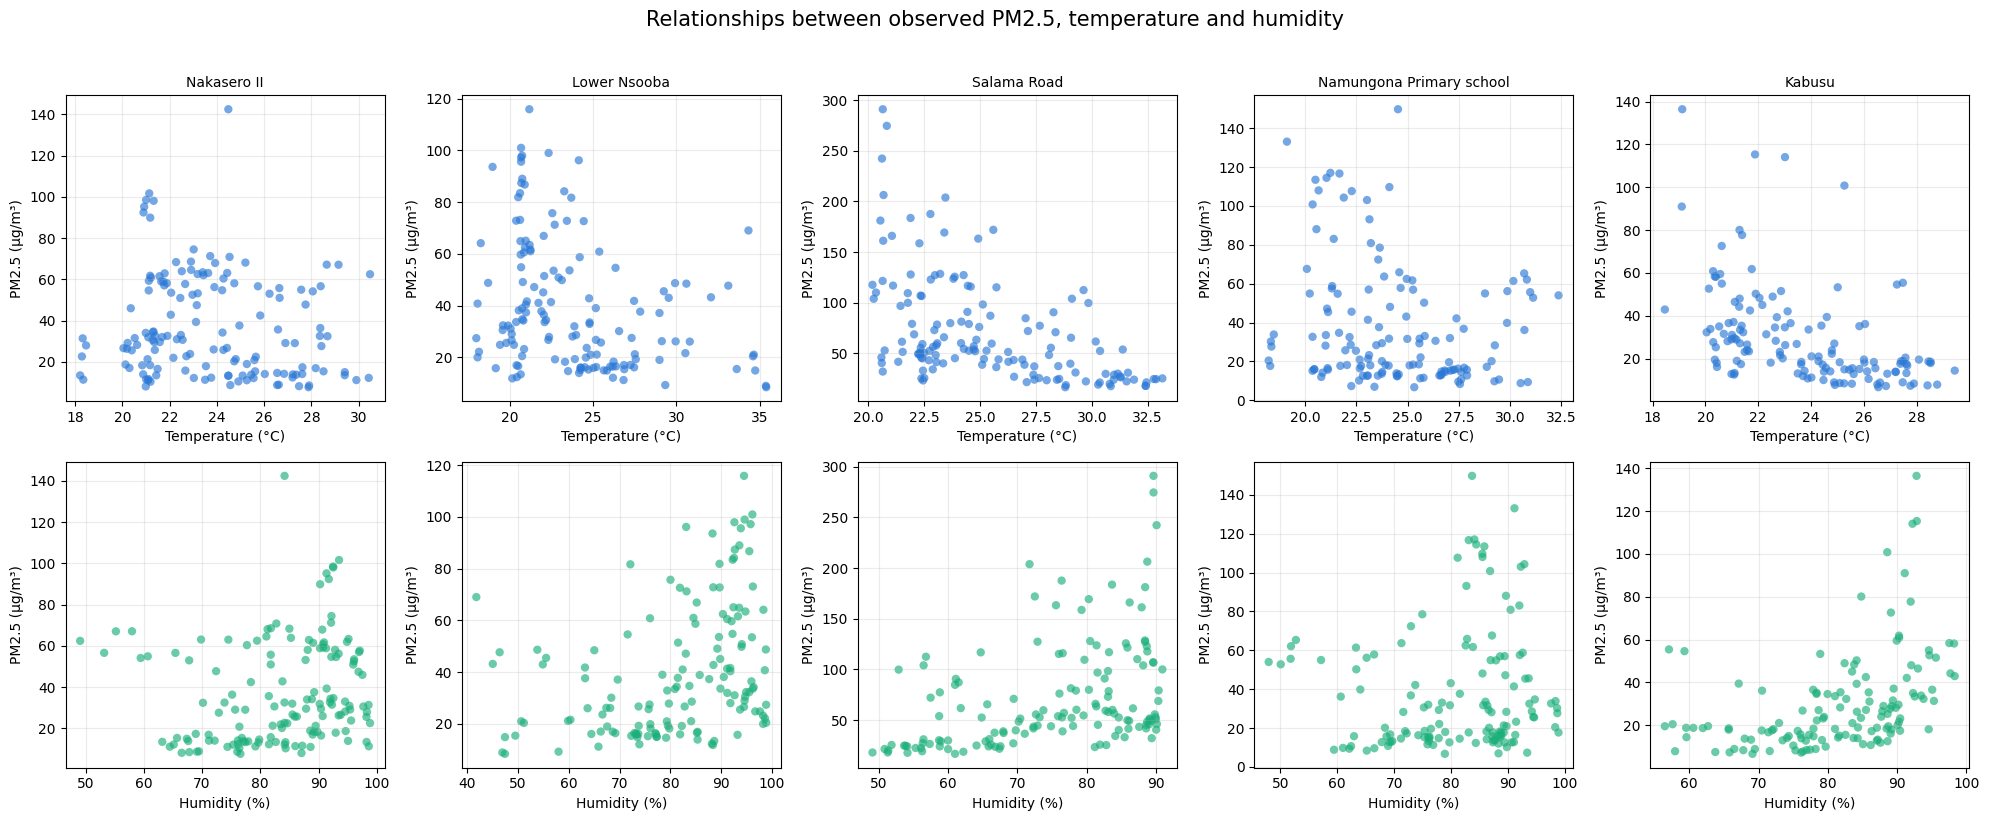
\includegraphics[width=\textwidth]{eda_scatter.png}
\caption{PM2.5 against temperature (top) and humidity (bottom) for each Kampala sensor.}
\label{fig:scatter}
\end{figure}

\begin{figure}[H]
\centering
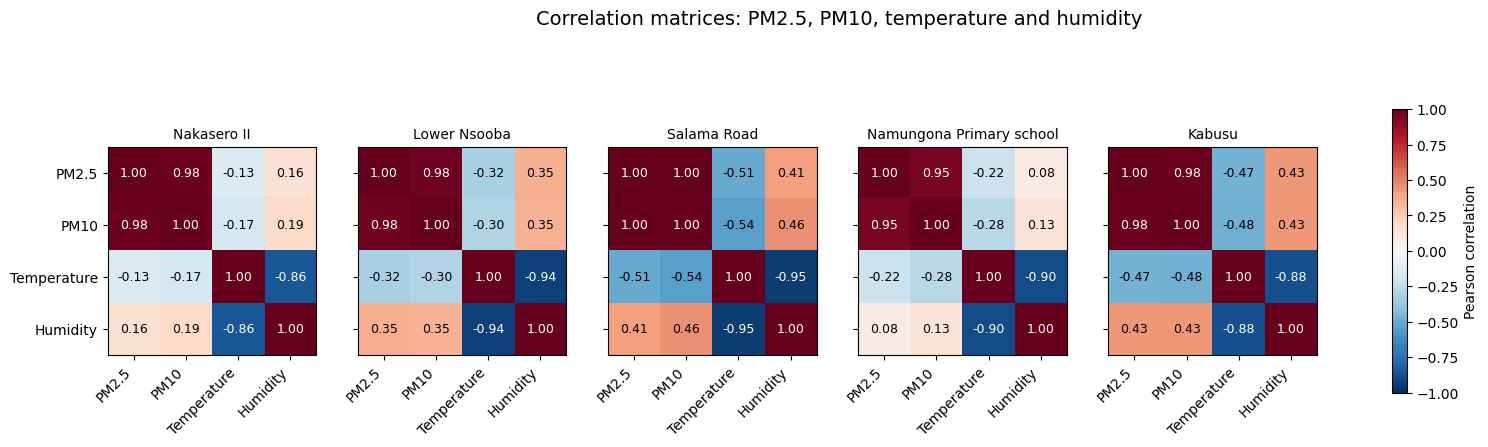
\includegraphics[width=\textwidth]{eda_correlation_matrices.png}
\caption{Correlation matrices of PM2.5, PM10, temperature and humidity for each Kampala sensor.}
\label{fig:corrmat}
\end{figure}

\subsection{Z-score transformation}

PM2.5 was standardised as $z = (x - \mu)/\sigma$ with $\mu = 32.71$\ugm{} and $\sigma = 30.36$\ugm, computed on genuine readings only, with zero and negative values excluded first (there were none in PM2.5). By construction the transformed series has mean 0 and standard deviation 1. A Z-score says how many standard deviations a reading sits from the network-wide average: $z = 1$ corresponds to 63.1\ugm{} (Unhealthy), and $z = -0.5$ to 17.5\ugm{} (Moderate). The median Z-score is $-0.39$, below zero, because the right-skewed tail pulls the mean above the typical reading. The maximum, $z = 31.8$, is the suspicious 998.4\ugm{} reading. Standardisation changes the scale but not the shape (Figure~\ref{fig:z}), so the skew remains. For modelling, the same transform is refitted on the training period only (Section~\ref{sec:setup}) to avoid leakage.

\begin{figure}[H]
\centering
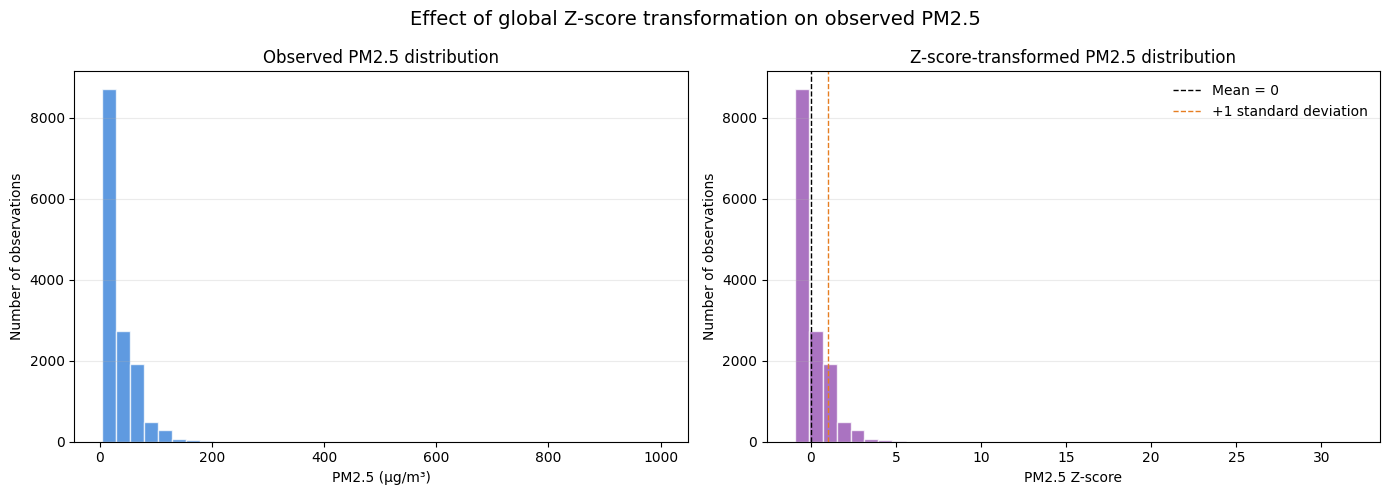
\includegraphics[width=0.95\textwidth]{eda_zscore.png}
\caption{Observed PM2.5 before and after the Z-score transformation.}
\label{fig:z}
\end{figure}

%==================================================================== 6
\section{Model implementation}

\subsection{Set-up}
\label{sec:setup}

\begin{itemize}
\item \textbf{Rows:} the 14{,}275 hours with a genuine PM2.5 reading. Resampled offline rows are never used as training targets.
\item \textbf{Chronological split:} training on 1 January -- 1 June (11{,}633 rows), testing on 2--3 June (2{,}642 rows). A random split would leak information from neighbouring hours into training and overstate accuracy.
\item \textbf{Target:} the Z-score of PM2.5, with mean (34.49\ugm) and standard deviation (31.70\ugm) fitted on the training period only. Predictions are inverse-transformed to \ugm{} for reporting.
\item \textbf{Preprocessing}, inside each model pipeline, so it is fitted on training data only: missing numeric inputs encoded as 0 and standardised; \texttt{device\_name} one-hot encoded, with unseen devices ignored.
\item \textbf{Tuning:} \texttt{GridSearchCV} or \texttt{RandomizedSearchCV} with \texttt{TimeSeriesSplit}, so every validation fold is later in time than its training fold. The test period is touched only once, for the final evaluation.
\end{itemize}

\subsection{Evaluation metrics}

\begin{itemize}
\item \textbf{MAE} (mean absolute error) is the primary selection metric: it is the average error in \ugm, easy to explain to non-technical stakeholders, and robust to the few extreme readings.
\item \textbf{RMSE} squares errors before averaging, so it penalises large misses. That matters here because missing a pollution spike is worse than a small error on a clean day.
\item \textbf{$R^2$} gives the share of variance explained, a scale-free summary of fit.
\item \textbf{AQI category accuracy} measures how often the predicted category matches the actual one, which is what the public sees.
\end{itemize}

MAPE was not used because it is unstable at low concentrations. If the goal were only to issue warnings, a classification metric such as recall on the Unhealthy-and-above categories would be more appropriate than any regression metric.

\subsection{Models and hyperparameters}

Six models were trained with scikit-learn~\cite{pedregosa2011}, covering the three groups in our approach report: five distinct models plus the Random Forest ensemble~\cite{breiman2001} (Table~\ref{tab:hyper}).

\begin{table}[H]
\centering
\caption{Models, tuned hyperparameters and why they matter.}
\label{tab:hyper}
\small
\begin{tabularx}{\textwidth}{l l L l}
\toprule
Model & Tuned & Why it matters & Selected \\
\midrule
Linear Regression & \texttt{fit\_intercept} & Whether the model estimates a baseline level or is forced through the origin; the reference model & True \\
Polynomial Regression & \texttt{degree} $\in\{1,2,3\}$ & Degree controls curvature: higher degrees fit non-linear weather effects but overfit & 1 \\
Ridge Regression & \texttt{alpha} & L2 penalty strength; stabilises coefficients of correlated inputs (temperature and humidity, $r \approx -0.9$) & 100 \\
Random Forest (ensemble) & \texttt{n\_estimators}, \texttt{max\_depth}, \texttt{min\_samples\_split}, \texttt{min\_samples\_leaf}, \texttt{max\_features} & More trees reduce variance; depth and leaf limits stop trees memorising noise; \texttt{max\_features} decorrelates the trees & 100 trees, depth 20, split 5, leaf 1, features 0.5 \\
SVR (RBF kernel) & \texttt{C}, \texttt{epsilon}, \texttt{gamma} & \texttt{C} trades margin against fit; \texttt{epsilon} sets the error-free tube; \texttt{gamma} sets how local the fit is & $C=5$, $\epsilon=0.2$, \texttt{auto} \\
KNN & \texttt{n\_neighbors}, \texttt{weights}, \texttt{p} & Few neighbours fit noise, many over-smooth spikes; \texttt{p} chooses Manhattan or Euclidean distance & 25, uniform, Manhattan \\
\bottomrule
\end{tabularx}
\end{table}

\subsection{Results}

\begin{table}[H]
\centering
\caption{Test-set results (2--3 June 2026), sorted by MAE.}
\label{tab:results}
\begin{tabular}{lrrr}
\toprule
Model & MAE (\ugm) & RMSE (\ugm) & $R^2$ \\
\midrule
\textbf{Random Forest (tuned)} & \textbf{3.103} & \textbf{7.003} & \textbf{0.898} \\
Random Forest (untuned baseline) & 3.272 & 7.123 & 0.894 \\
SVR (tuned) & 4.585 & 7.697 & 0.877 \\
Ridge Regression (tuned) & 5.292 & 9.923 & 0.795 \\
KNN (tuned) & 5.722 & 11.670 & 0.716 \\
Polynomial Regression (tuned) & 6.005 & 10.606 & 0.766 \\
Linear Regression (tuned) & 6.005 & 10.606 & 0.766 \\
\bottomrule
\end{tabular}
\end{table}

Table~\ref{tab:results} shows that the tuned Random Forest is the best model on every metric. It was selected and serialised (\texttt{best\_pm25\_model.joblib}, with the target scaler and feature lists). Tuning improved it over the untuned baseline by 0.17\ugm{} MAE. Polynomial Regression chose degree 1 and is therefore identical to Linear Regression: cross-validation found no benefit from added curvature. Tree ensembles also suit the approach report's requirement that the model tolerate missing inputs gracefully.

\textbf{AQI categories.} Converted to categories, 86.2\% of test hours are classified correctly (Figure~\ref{fig:conf}). Nearly all errors are one category away. The most common error is ``Good'' hours predicted as ``Moderate'' (205 of 269), so at the low end the model leans towards over-warning. All 20 Very Unhealthy hours were predicted as Unhealthy or worse.

\begin{figure}[H]
\centering
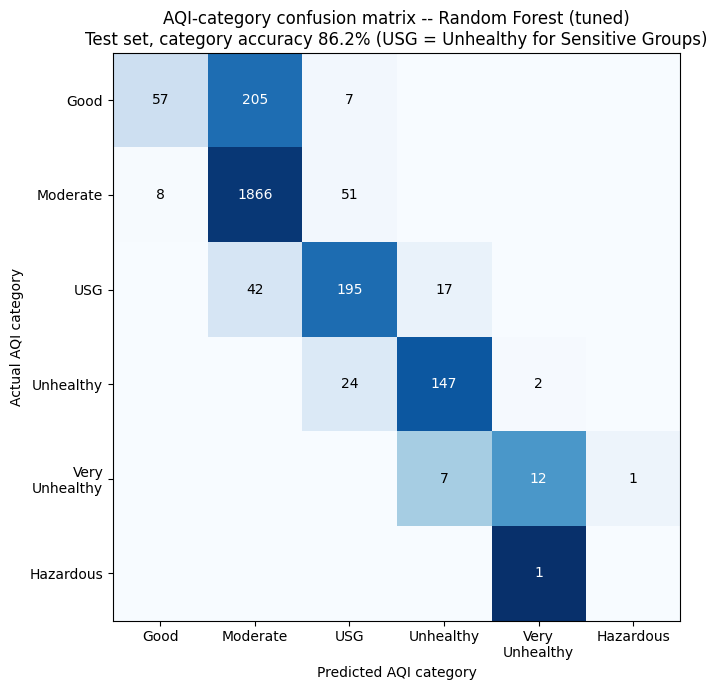
\includegraphics[width=0.62\textwidth]{model_aqi_confusion.png}
\caption{Confusion matrix of AQI categories for the selected model on the test set.}
\label{fig:conf}
\end{figure}

\subsection{What drives the accuracy}
\label{sec:importance}

Table~\ref{tab:importance} shows the Random Forest's feature importances. PM10 alone carries 76\%. This matches the near-perfect PM2.5--PM10 correlation in the EDA: both come from the same optical sensor at the same moment.

\begin{table}[H]
\centering
\caption{Feature importance of the selected Random Forest (one-hot device columns summed).}
\label{tab:importance}
\begin{tabular}{lr}
\toprule
Feature & Importance \\
\midrule
PM10 & 75.7\% \\
Device (149 one-hot columns) & 12.4\% \\
Month (cos) & 4.7\% \\
Hour (cos and sin) & 3.2\% \\
Temperature & 1.4\% \\
Day of week (cos and sin) & 1.3\% \\
Humidity & 0.8\% \\
Month (sin) & 0.5\% \\
\bottomrule
\end{tabular}
\end{table}

To understand how much of the model's skill would survive in a true forecasting setting, where PM10 is not known in advance, we retrained a Random Forest on reduced feature sets (Table~\ref{tab:sens}). Without PM10, test $R^2$ falls from 0.90 to about 0.15. With only temperature, humidity and time (no PM10, no device, genuine weather readings only), no model beat simply predicting the training median. This is consistent with Febrian and Permai~\cite{febrian2025}, who found that past pollutant values alone were sufficient for short-term PM2.5 forecasting and that meteorology added little.

\begin{table}[H]
\centering
\caption{Sensitivity of test accuracy to the feature set (Random Forest, same chronological split).}
\label{tab:sens}
\begin{tabular}{lrr}
\toprule
Features & MAE (\ugm) & $R^2$ \\
\midrule
Weather + PM10 + time + device & 3.32 & 0.899 \\
Weather + time + device (no PM10) & 11.20 & 0.133 \\
Time + device only & 11.12 & 0.175 \\
Weather + time only, genuine weather rows only (best of six models) & 14.38 & $-0.05$ \\
Baseline on the same rows: always predict the training median & 13.56 & $-0.08$ \\
\bottomrule
\end{tabular}
\end{table}

%==================================================================== 7
\section{Forecasting and visualisation}

The saved model produced daily forecasts for all 149 sensors for 1--14 August 2026 (2{,}086 sensor-days) and hourly forecasts for 1 August 2026 (3{,}576 sensor-hours). Predictions are made on the Z-score scale and inverse-transformed to \ugm. Daily values are the mean of the 24 hourly predictions.

August lies entirely outside the data, so the time features are computed from the forecast timestamps, while temperature, humidity and PM10 had to be estimated. Each sensor's own historical average for that hour of the day (its diurnal climatology) was used, falling back to the all-sensor average for that hour. All forecasts are produced in a single pass, not step by step, so the two-week horizon takes under a second. All forecast checks passed: correct row counts, all 149 sensors and 14 days, and no missing or negative predictions.

Across all sensor-days, 1{,}356 are forecast as Moderate, 490 Unhealthy for Sensitive Groups, 226 Unhealthy and 14 Very Unhealthy; none are Good. Hourly, the early-morning and evening hours carry the highest values. Figures~\ref{fig:fccal} and~\ref{fig:fcts} show the daily forecasts for the five Kampala sensors with the AQI legend.

\begin{figure}[H]
\centering
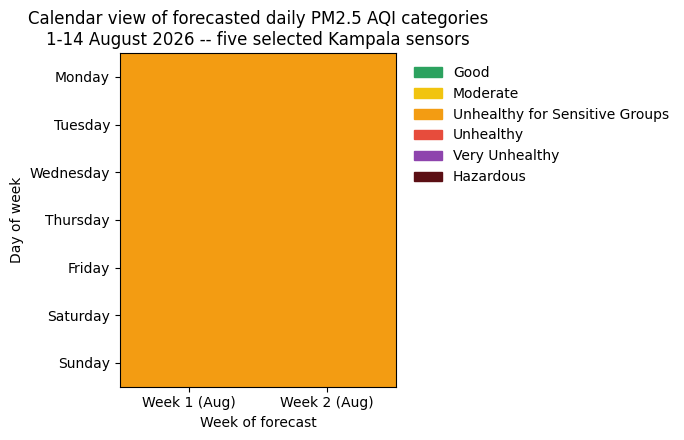
\includegraphics[width=0.75\textwidth]{forecast_calendar.png}
\caption{Calendar of forecast daily PM2.5 for 1--14 August 2026 (mean of the five Kampala sensors), coloured by AQI category.}
\label{fig:fccal}
\end{figure}

\begin{figure}[H]
\centering
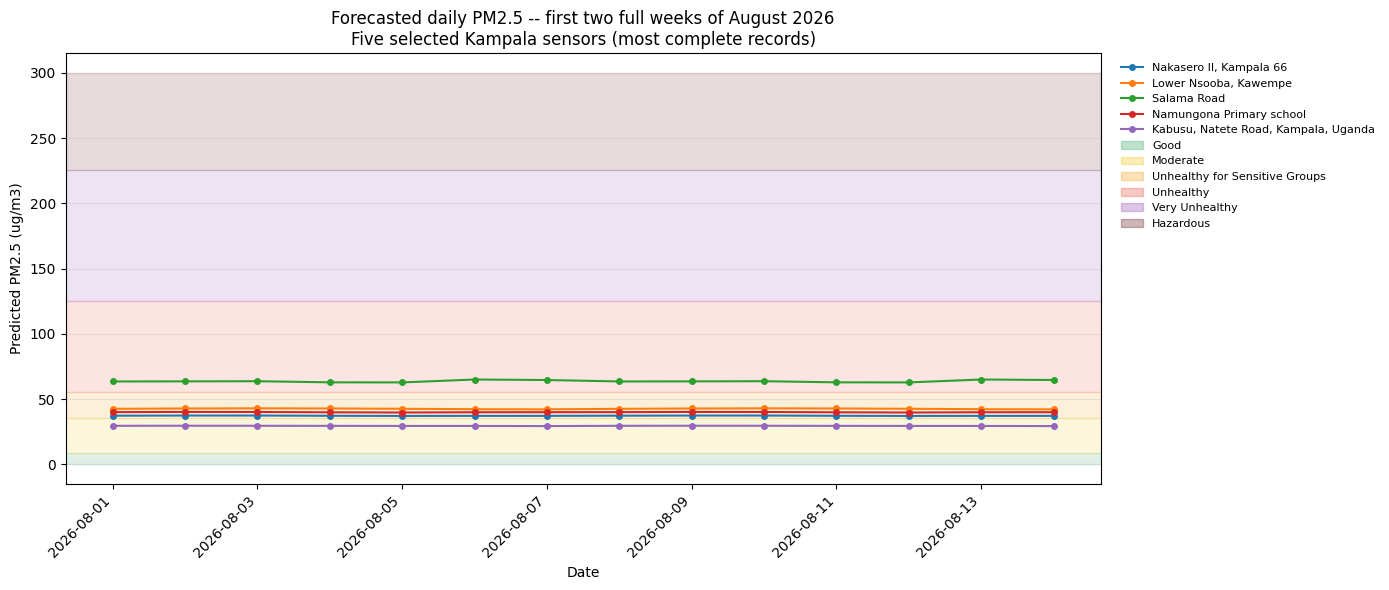
\includegraphics[width=\textwidth]{forecast_timeseries.png}
\caption{Forecast daily PM2.5 for the five Kampala sensors, 1--14 August 2026, with AQI bands.}
\label{fig:fcts}
\end{figure}

\textbf{Interpretation and limits.} Because the weather and PM10 inputs are typical values rather than real August observations, the forecasts repeat each sensor's typical weekly pattern. They indicate which sites are usually worse (for example Salama Road), not what will happen on a particular day. Given Table~\ref{tab:sens}, forecast accuracy on real future days should be expected to be much lower than the test MAE of 3.1\ugm.

The optional shapefile map of sensors in the USG and Very Unhealthy range at 13:00 on 1 August was not attempted, because no shapefile was available. The underlying predictions are in the hourly forecast file.

%==================================================================== 8
\section{Model monitoring with Evidently AI}

Evidently 0.7.23~\cite{evidently} compares a \emph{reference} dataset, the training period (11{,}633 rows), with a \emph{current} dataset, the test period (2{,}642 rows), as a stand-in for live data. Two reports were generated: a data-drift report on the inputs and a regression report on the predictions. The Evidently cells are wrapped so that an Evidently error cannot crash the pipeline, as the brief requires. The pipeline was also verified with Evidently switched off.

\subsection{Data drift}

For each feature, Evidently compares the reference and current distributions and reports a \textbf{drift score}:
\begin{itemize}
\item \textbf{Normed Wasserstein distance} (numeric features): the ``earth mover's'' distance between the two distributions, divided by the reference standard deviation. A value of 0.1 means the distribution moved by about a tenth of a standard deviation.
\item \textbf{Jensen--Shannon distance} (categorical or low-cardinality features): a symmetric measure of difference between two category distributions, from 0 (identical) to 1 (no overlap).
\item \textbf{Threshold:} a feature is flagged as drifting when its score is at least 0.1.
\item \textbf{Drifted columns count and share:} the number and fraction of features that drifted. The dataset as a whole is declared drifting when the share reaches 0.5.
\end{itemize}

\begin{figure}[H]
\centering
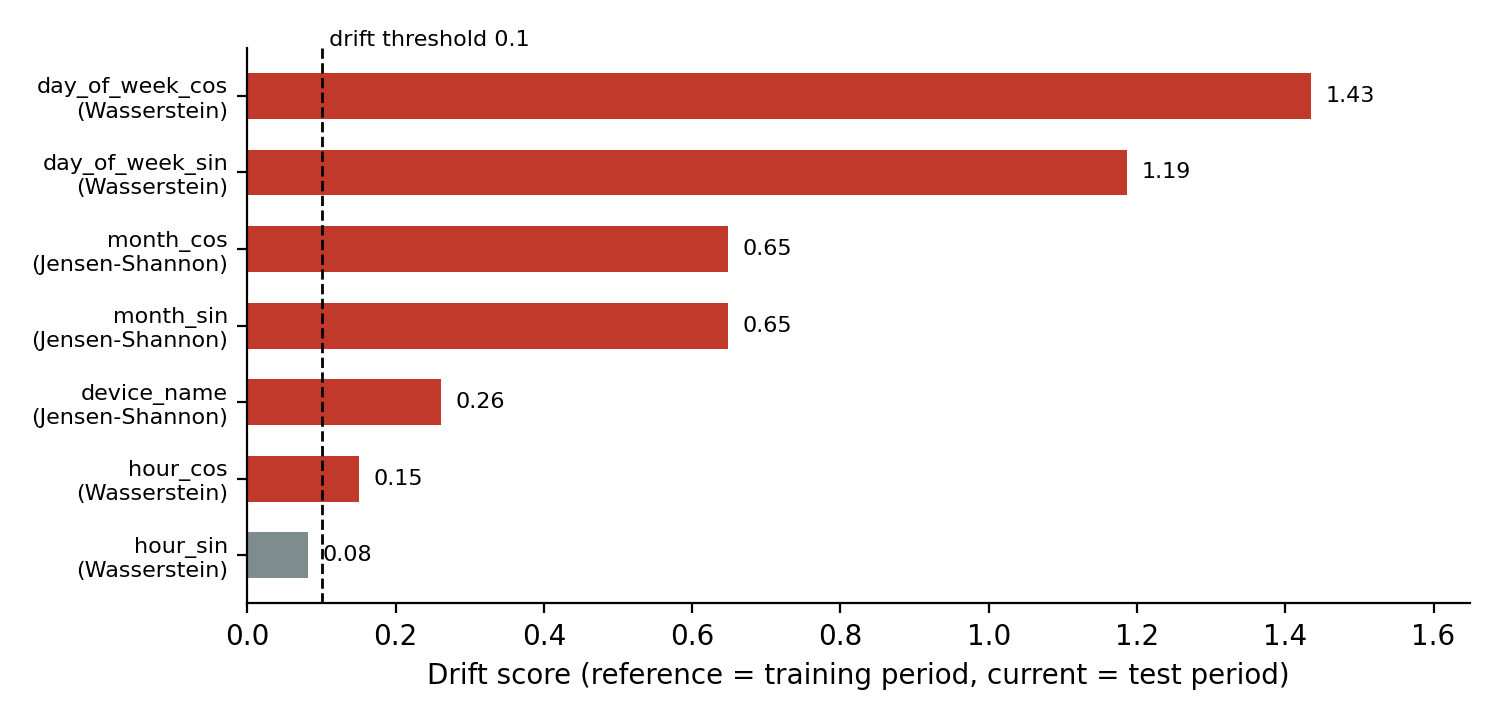
\includegraphics[width=0.85\textwidth]{monitoring_drift_scores.png}
\caption{Evidently drift scores, training period vs.\ test period. Red bars exceed the 0.1 threshold.}
\label{fig:drift}
\end{figure}

Six of seven scored features drifted (share 0.86 $\ge$ 0.5), so Evidently declares dataset drift (Figure~\ref{fig:drift}). The cause is the composition of the windows, not a change in the air. The test window contains only two weekdays of one month, so the day-of-week (1.43 and 1.19) and month (0.65) features necessarily differ from training. Only 119 of the 149 training sensors report in June, hence device drift (0.26). Hour-of-day barely moved (0.08 and 0.15). For this pipeline, the alert means ``the current data is not representative of what the model was trained on'' rather than ``pollution behaviour has changed''. In production, the same check run weekly would flag a broken or missing sensor group early.

Evidently did not produce drift scores for temperature, humidity and PM10. These columns use pandas' nullable \texttt{Float64} type, which Evidently did not recognise as numeric. We therefore monitored them separately: their missingness fell from 29.8\% to 15.6\% (temperature) and from 31.5\% to 16.0\% (humidity) between the periods, and their spread narrowed. Converting these columns to standard \texttt{float64} before building the report would include them; this is a known fix for the next iteration.

\subsection{Model drift}

\begin{table}[H]
\centering
\caption{Model performance, reference (training) period vs.\ current (test) period.}
\label{tab:modeldrift}
\begin{tabular}{lrrr}
\toprule
Period & MAE (\ugm) & RMSE (\ugm) & $R^2$ \\
\midrule
Reference (training, in-sample) & 1.92 & 6.14 & 0.962 \\
Current (test) & 3.10 & 7.00 & 0.898 \\
\bottomrule
\end{tabular}
\end{table}

The regression report tracks MAE, RMSE, $R^2$, mean error (bias) and the distribution of errors. Error rises from reference to current (Table~\ref{tab:modeldrift}). Part of this is expected, because reference predictions are in-sample. The mean prediction (24.6\ugm) stays close to the mean actual value (24.8\ugm), so the model is not systematically biased on new data. In production, a sustained rise in MAE on newly labelled readings, beyond what is seen here, would trigger retraining. Our approach report also specifies keeping the previous model checkpoint and rolling back if a retrain validates worse.

%==================================================================== 9
\section{Deployment}

\subsection{Choice of cloud platform}

The brief proposed RunPod, a pay-as-you-go GPU cloud, with a budget of up to \$5. We first planned the deployment there: we sized a Pod (one RTX 2000 Ada GPU, 6 vCPU, 31\,GB RAM, PyTorch template) and prepared an automated run script. However, RunPod requires credit to be bought in advance before any Pod can start. That upfront payment became financially straining for the group, so we moved the deployment to \textbf{Kaggle}, which provides free cloud notebooks.

Kaggle suits this pipeline well. Our measurements (Section~\ref{sec:local}) show the pipeline is CPU-only (scikit-learn), needs about 1\,GB of RAM, and finishes in about 11 minutes. That is well within Kaggle's free CPU sessions, so no GPU or paid tier is needed. Kaggle runs a saved notebook as a batch job in the cloud (``Save \& Run All''), and keeps each run's log and output files with the saved version. These are exactly the runtime logs and metrics the brief asks us to check.

\subsection{Local verification}
\label{sec:local}

As the brief requires, the pipeline was first run cleanly end to end locally with the pinned package versions in \texttt{requirements.txt} (Table~\ref{tab:local}). Resource needs were measured rather than estimated, and inference was measured separately from training, as set out in our approach report.

\begin{table}[H]
\centering
\caption{Local verification (Windows 11, Python 3.13, 16 logical CPUs).}
\label{tab:local}
\begin{tabularx}{\textwidth}{l L}
\toprule
Check & Result \\
\midrule
Full notebook run & All cells executed, 0 errors \\
Run with Evidently switched off & All cells executed, 0 errors \\
Pipeline runtime & 662\,s (11.0 min), single-threaded model tuning \\
Peak RAM & 988 MB \\
Model artifact & 115 MB; reloads in a fresh process in 0.5\,s \\
Prediction latency & 1 row: 22\,ms; 3{,}576 rows: 98\,ms; 50{,}064 rows: 730\,ms \\
Forecast mode & Single pass over all forecast rows (not autoregressive) \\
Standalone inference script & Identical predictions to the notebook on all 2{,}642 test rows \\
\bottomrule
\end{tabularx}
\end{table}

\subsection{Deployment on Kaggle}

The deployment steps were:
\begin{enumerate}
\item import \texttt{train.ipynb} into a new Kaggle notebook;
\item attach the sensor CSV as a Kaggle dataset (the notebook finds it under \texttt{/kaggle/input} automatically);
\item install the pinned package versions;
\item run the whole pipeline in the cloud with \emph{Save \& Run All}: data import, cleaning, EDA, training and tuning, forecasting, Evidently monitoring and model packaging.
\end{enumerate}

The final notebook section records the \textbf{runtime log and resulting metrics} of the cloud run. It saves them to \texttt{kaggle\_run\_log.txt} and \texttt{kaggle\_run\_metrics.json} in the run's output: platform and hardware, start and end time, runtime, peak memory, the rows at each pipeline stage, every model's test scores, the selected model's metrics and AQI accuracy, the forecasts and the monitoring result. Table~\ref{tab:kaggle} summarises the Kaggle run.

\begin{table}[H]
\centering
\caption{Runtime log and resulting metrics of the Kaggle run (from \texttt{kaggle\_run\_log.txt}).}
\label{tab:kaggle}
\begin{tabularx}{\textwidth}{l L}
\toprule
Item & Kaggle run \\
\midrule
Hardware (CPUs, RAM, GPU) & \tofill{CPUs / RAM / GPU line} \\
Start and end time (UTC) & \tofill{Started / Finished lines} \\
Pipeline runtime & \tofill{Runtime line} \\
Peak RAM & \tofill{Peak RAM line} \\
Rows: raw / training / test & 14{,}600 / 11{,}633 / 2{,}642 \tofill{confirm from Pipeline stages} \\
Selected model & \tofill{Selected model line} \\
Test MAE / RMSE / $R^2$ & \tofill{expected 3.103 / 7.003 / 0.898} \\
AQI category accuracy & \tofill{expected 86.2\%} \\
Forecasts & \tofill{expected 2{,}086 daily and 3{,}576 hourly rows} \\
Evidently monitoring & \tofill{Evidently line} \\
Prediction latency & \tofill{Latency line} \\
Cost & Free (Kaggle notebook) \\
\bottomrule
\end{tabularx}
\end{table}

% To add a screenshot of the Kaggle run, save it as figures/kaggle_run.png and uncomment:
% \begin{figure}[H]
% \centering
% \includegraphics[width=\textwidth]{kaggle_run.png}
% \caption{The pipeline's run log at the end of the Kaggle run.}
% \label{fig:kaggle}
% \end{figure}

The run also produces the deployment artifacts. The serialised model, with its target scaler and feature lists, was validated by reloading it in a fresh Python process. A standalone script (\texttt{pm25\_inference.py}) produces batch predictions from a CSV of features; it reproduced the notebook's predictions exactly.

\subsection{Demo on Hugging Face}

To make the results accessible beyond the notebook, we published:
\begin{itemize}
\item the trained model, with a model card describing its inputs, metrics, usage and limitations, at \url{https://huggingface.co/Kyalis/airqo-pm25-random-forest};
\item an interactive demo page as a Hugging Face Space at \url{https://huggingface.co/spaces/Kyalis/airqo-pm25-forecasts} (Figures~\ref{fig:hfdaily} and~\ref{fig:hfhourly}). A visitor chooses any of the 149 sensors and sees its 14-day AQI calendar and hourly forecast for 1 August, coloured by AQI category.
\end{itemize}

\begin{figure}[H]
\centering
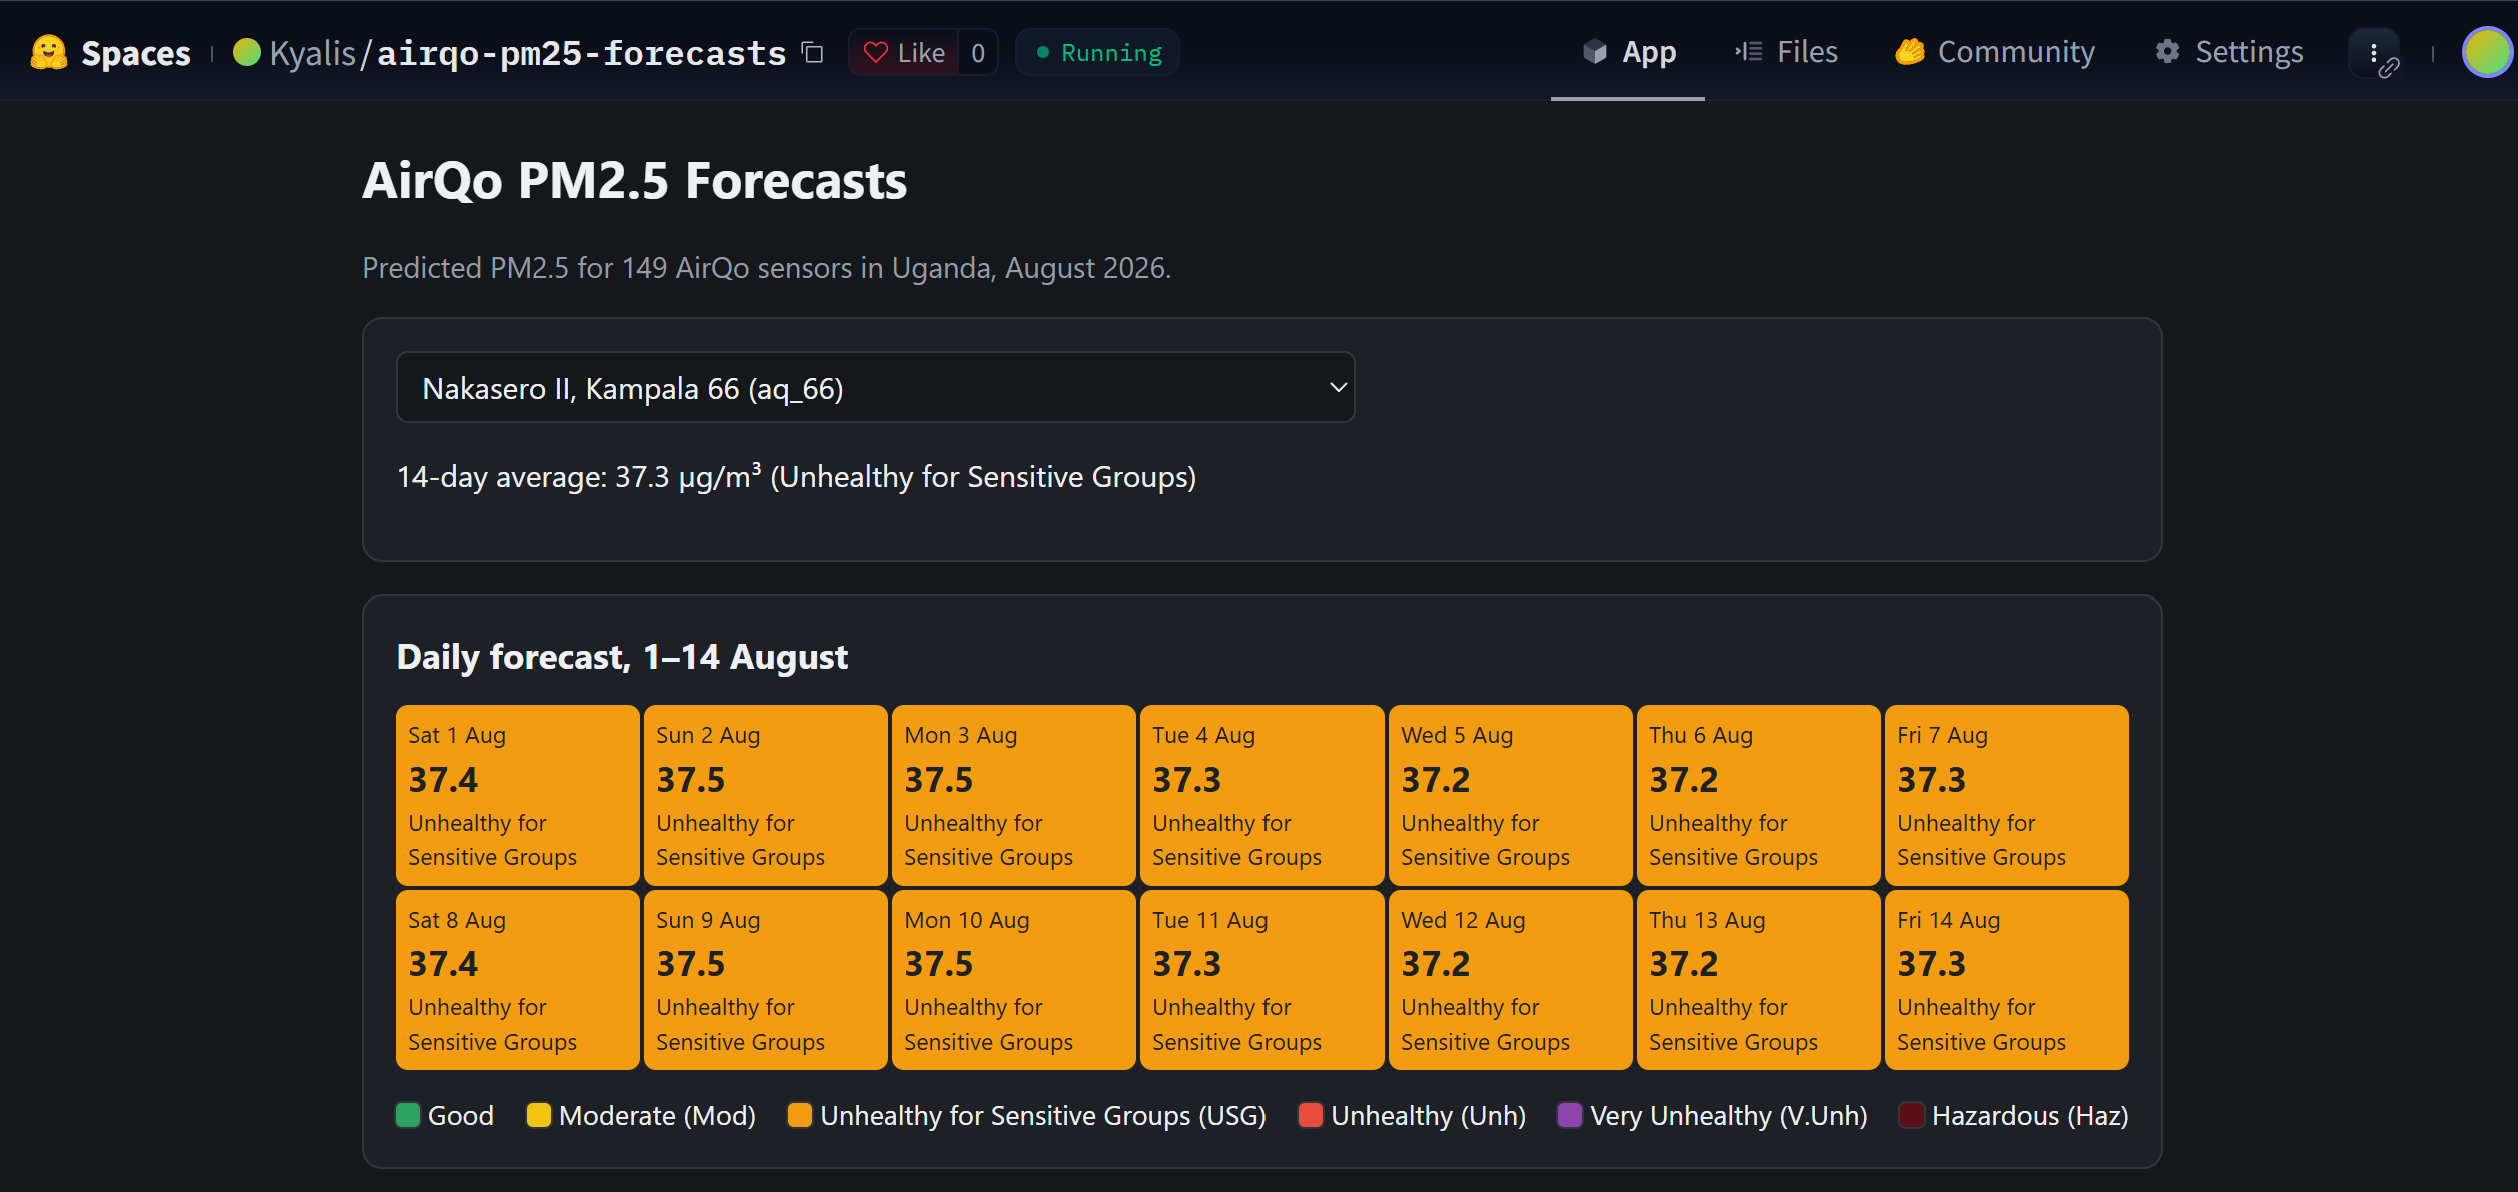
\includegraphics[width=\textwidth]{hf_space_daily.png}
\caption{Hugging Face demo: sensor selection, 14-day average and the daily AQI calendar for 1--14 August 2026.}
\label{fig:hfdaily}
\end{figure}

\begin{figure}[H]
\centering
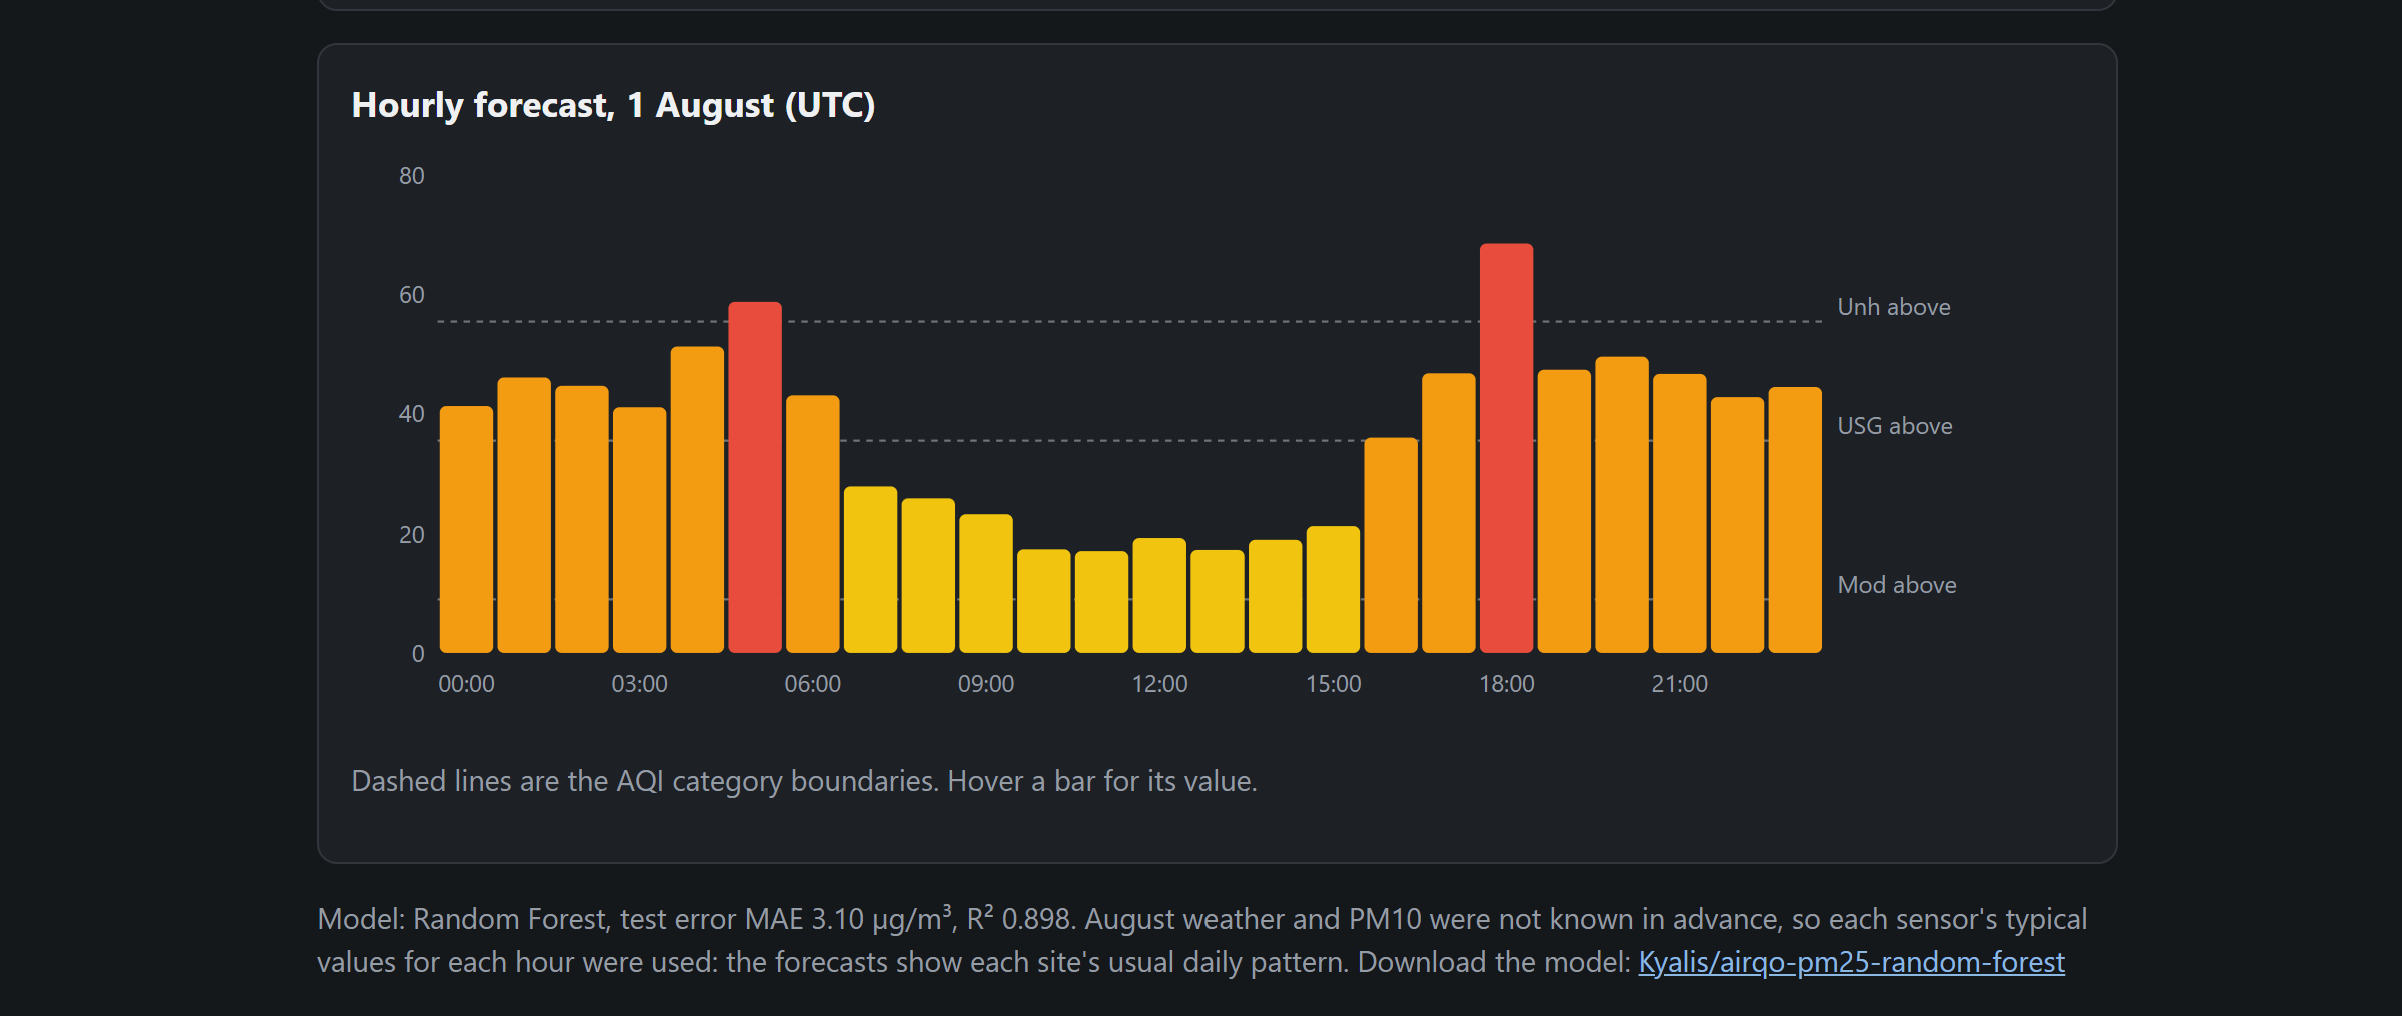
\includegraphics[width=\textwidth]{hf_space_hourly.png}
\caption{Hugging Face demo: hourly forecast for 1 August 2026 with AQI category boundaries.}
\label{fig:hfhourly}
\end{figure}

\textbf{Limitation: no live inference on Hugging Face.} The demo shows the forecasts produced by the pipeline; it does not run the model itself. Hugging Face only allows free accounts to host \emph{static} Spaces (HTML and JavaScript). Spaces that run Python on a server (Gradio or Docker), which would be needed to load the scikit-learn model and predict on request, require a paid PRO subscription on the free CPU tier. Our attempts to create such a Space were refused with an HTTP 402 ``Payment Required'' error. As future work (Section~\ref{sec:future}), we would convert the model to the ONNX format, so that the static page could run the real model directly in the visitor's browser with ONNX Runtime Web.

%==================================================================== 10
\section{Discussion and limitations}

\begin{itemize}
\item \textbf{Little data in time.} Eight days in three months cannot capture seasonal patterns, and the test period is just over a day. The test metrics describe a short window and should be read with that in mind.
\item \textbf{PM10 dependence.} The high accuracy relies on PM10 measured at the same hour. For genuine forecasting, the most promising improvement is to add lagged PM2.5 and PM10 (for example the readings 24 hours earlier) and real or forecast weather. This is consistent with the Jakarta study~\cite{febrian2025}.
\item \textbf{Sensor quality.} PM2.5 exceeding PM10 in 22\% of rows, and suspicious extremes such as 998\ugm, suggest calibration issues worth reporting to AirQo. These rows were flagged rather than removed.
\item \textbf{Monitoring coverage.} The weather and PM10 columns need a type conversion to be included in Evidently's drift report.
\item \textbf{No live inference in the demo.} The Hugging Face page displays the pipeline's forecasts rather than running the model, because server-side Spaces are not free.
\end{itemize}

\subsection{Future development}
\label{sec:future}

\begin{itemize}
\item \textbf{Managed cloud deployment on GCP or Azure.} For production we would consider Google Cloud Platform or Microsoft Azure. On GCP, the model could be served from a container on Cloud Run or as a Vertex AI endpoint, with the pipeline scheduled to retrain on new AirQo data. On Azure, the equivalent services are Azure Machine Learning managed online endpoints, or Azure Container Apps. Both offer student credits, autoscaling, and built-in logging and monitoring. Our prediction API (\texttt{serve\_model.py}, \texttt{GET /health} and \texttt{POST /predict}) is ready to be packaged as a container for either platform.
\item \textbf{In-browser inference with ONNX.} Converting the trained pipeline to ONNX would let the free static Hugging Face page run the real model in the visitor's browser with ONNX Runtime Web, so users could enter their own weather and PM10 values and get live predictions at no hosting cost.
\item \textbf{Better forecasting inputs.} Add lagged pollutant readings and weather forecasts, so the model can predict genuinely unseen future days.
\item \textbf{Automated monitoring and rollback.} Run the Evidently reports on a schedule against newly arriving data, retrain when error grows, and keep the previous model checkpoint to roll back to if a retrain validates worse, as planned in our approach report.
\end{itemize}

%==================================================================== 11
\section{Conclusion}

We delivered a reproducible pipeline that cleans and resamples the AirQo data without inventing PM2.5 targets, explores it with AQI-coloured visualisations, and trains and tunes six regression models on a leakage-safe chronological split. The selected tuned Random Forest achieves MAE 3.10\ugm{} and $R^2$ 0.898 on held-out data, and 86.2\% AQI category accuracy. It produced the required August forecasts and is monitored with Evidently. The full pipeline was deployed and run in the cloud on Kaggle, after RunPod's prepaid credits proved too costly for the group, and the model and an interactive forecast demo were published on Hugging Face. The main lesson is that the model's skill comes from PM10 measured at the same time: true forward forecasting will need past pollutant readings and weather forecasts as inputs. Managed services on GCP or Azure are the natural next step for a production deployment.

%==================================================================== Refs
\begin{thebibliography}{9}

\bibitem{febrian2025}
S.~Febrian and S.~D.~Permai.
\newblock PM2.5 index prediction in Central Jakarta using pollution and meteorological data with CNN-LSTM.
\newblock \emph{E3S Web of Conferences}, 680:00067, 2025.
\newblock \url{https://doi.org/10.1051/e3sconf/202568000067}.

\bibitem{okure2022}
D.~Okure, J.~Ssematimba, R.~Sserunjogi, N.~L.~Gracia, M.~E.~Soppelsa and E.~Bainomugisha.
\newblock Characterization of ambient air quality in selected urban areas in Uganda using low-cost sensing and measurement technologies.
\newblock \emph{Environmental Science \& Technology}, 56(6):3324--3339, 2022.
\newblock \url{https://doi.org/10.1021/acs.est.1c01443}.

\bibitem{sserunjogi2022}
R.~Sserunjogi, J.~Ssematimba, D.~Okure, D.~Ogenrwot, P.~Adong, L.~Muyama, N.~Nsimbe, M.~Bbaale and E.~Bainomugisha.
\newblock Seeing the air in detail: hyperlocal air quality dataset collected from spatially distributed AirQo network.
\newblock \emph{Data in Brief}, 44:108512, 2022.

\bibitem{who2021}
World Health Organization.
\newblock \emph{WHO Global Air Quality Guidelines: Particulate Matter (PM2.5 and PM10), Ozone, Nitrogen Dioxide, Sulfur Dioxide and Carbon Monoxide}.
\newblock Geneva: WHO, 2021.

\bibitem{breiman2001}
L.~Breiman.
\newblock Random forests.
\newblock \emph{Machine Learning}, 45(1):5--32, 2001.

\bibitem{pedregosa2011}
F.~Pedregosa et al.
\newblock Scikit-learn: machine learning in Python.
\newblock \emph{Journal of Machine Learning Research}, 12:2825--2830, 2011.

\bibitem{evidently}
Evidently AI.
\newblock Evidently: open-source ML and data monitoring, version 0.7.23.
\newblock \url{https://github.com/evidentlyai/evidently}.

\end{thebibliography}

%==================================================================== Appendix
\appendix
\section{Reproducing the results}

\begin{tabularx}{\textwidth}{l L}
\toprule
File & Purpose \\
\midrule
\texttt{train.ipynb} & The full pipeline, from raw data to deployment outputs \\
\texttt{requirements.txt} & Pinned package versions (Python 3.11+) \\
\texttt{DEPLOYMENT.md} & Step-by-step instructions for running the pipeline on Kaggle \\
\texttt{serve\_model.py} & HTTP prediction endpoint (\texttt{GET /health}, \texttt{POST /predict}) \\
\texttt{pm25\_inference.py} & Command-line batch inference from a CSV of features \\
\texttt{best\_pm25\_model.joblib} & The trained model, target scaler and feature lists \\
\texttt{deployment\_outputs/} & August forecasts, metadata, resource report and the Kaggle run log \\
\texttt{evidently\_*.html} & Evidently data-drift and model-drift reports \\
\bottomrule
\end{tabularx}

To reproduce locally: \texttt{pip install -r requirements.txt}, then run all cells of \texttt{train.ipynb}, or execute it unattended with \texttt{jupyter nbconvert --to notebook --execute train.ipynb}. On Kaggle: follow \texttt{DEPLOYMENT.md}.

\end{document}
